\section{Weakly Hard Model and Control Systems} \label{application}

\subsection{Control Systems}
This section studies an example~\cite{liang2019security} to enhance the security and robustness of control systems by leveraging weakly hard constraints. We consider a feedback controller design for physical plants with linear time-invariant model. The dynamics of the system can be formulated by the following state-space model:
\begin{align*}
\dot{x}(t) &= Ax(t) + Bu(t) \\
y(t) &= Cx(t) + Du(t) \\
u(t) &= Ky(t)
\end{align*}
where x(t), y(t), and u(t) are vectors representing the states, the output, and the control input of the system at time t, respectively. A, B, and C are system matrices. 

This continuous model of control systems needs to be discretized before being implementing on digital platforms. We assume that computation delay and communication delay are negligible in the system. A typical model of such discrete system is as follows:
\begin{align*}
    z[k+1] &= A_{aug} z[k] + B_{aug} u[k] \\
    y[k] &= C_{aug} z[k] \\
    u[k] &= -Kz[k]
\end{align*}
where z[k], y[k], and u[k] denote the augmented states, the output, and the control input of the system at time $h_k$, respectively, where $h_k$ denotes the time t at the k-th cycle. K is the feedback gain of the system that ensures the stability of the system. $A_{aug}$  is a matrix $\in$ $\hspace{0.3mm}$ $R^n$ $\times$ $R^n$, $B_{aug}$  is a matrix $\in$$\hspace{0.3mm}$ $R^n$ $\times$ $1$, and $C_{aug}$ is a matrix $\in$ $\hspace{0.3mm}$ $1$ $\times$ $R^n$. 

\subsection{Stability and Control Performance} \label{stability and control performance}
To optimize the design of control systems under the weakly hard model, we need to study the impact of deadline miss pattern on the stability and control performance of the system. A discrete control system as described in the previous section is stable if all the closed-loop poles lie in the unit circle in a complex plane. This system dynamics is described as follows:
\begin{align*}
z[k + 1] &= (A_{aug} - B_{aug}K)z[k] \\
A_{cl} &= A_{aug} - B_{aug}K
\end{align*}
The stability property is formalized as a study of the eigenvalues of the matrix $A_{cl}$. The closed-loop system is stable if and only if all eigenvalues of $A_{cl}$ are within the unit circle in the complex plane, i.e. their lengths are all less than 1.

While stability considers whether the system can be stabilized, control performance measures how quickly the controller can bring the system back to the equilibrium state after a disturbance, assuming the the system can be stabilized. The control performance is quantified by a metric H. H stands for the minimal number of sampling cycles to bring a disturbance J back to a certain predefined threshold $J_{th}$. This property is formalized as the following equation:
\begin{align*}
 \forall r &\ge H \\
 &J_r \le J_th 
\end{align*}

\subsection{Weakly Hard Constraints} \label{weakly hard constraints formulation}
The weakly hard model we take into consideration in this example is the m-K model that allows a task to "misses any n in m deadlines" (Definition~\ref{def:missany}). We quantitively formalize this timing requirement for a task $\tau$ as
\begin{align*}
(k^{j}, N^{j})
\end{align*}
which represents that for a sequence of $N^{j}$ consecutive activations of task $\tau$, there are at most $k^{j}$ deadline misses. 

We also denote
\begin{align*}
dmm(N^j)
\end{align*}
as the number of deadline misses in the worst case for task $\tau$ in any sequence of $N^j$ consecutive activations.

With these notions in hand, we can formally define a task $\tau$ satisfying its weakly hard constraint $(k^{j}, N^{j})$ as follows:
\begin{align*}
dmm(N^j) \le k^j, \forall j
\end{align*}

\subsection{Security Monitoring Tasks}
The goal of this example ~\cite{liang2019security} is to improve the security of the embedded control systems by optimizing the allocation, priority, and period assignments of the security monitoring tasks leveraging the weakly hard constraints. Security monitoring tasks read the CAN messages to detect intrusion. Security monitoring tasks are periodic tasks. For each period, an activation of the security monitoring task reads the CAN messages it monitors and check for anomaly intrusions. Figure ~\ref{fig:system_model} shows a model of system with security monitoring tasks.

\begin{figure}[h!]
\caption{System model with security monitoring tasks~\cite{liang2019security}}
\centering
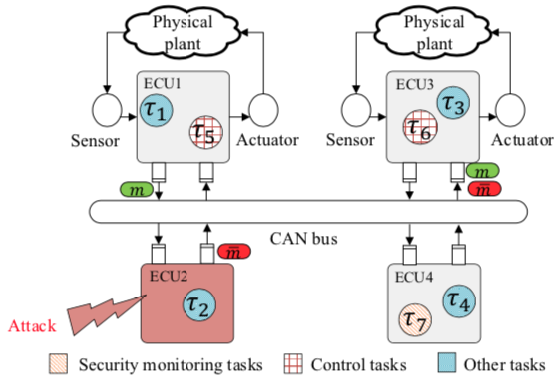
\includegraphics[width=0.5\textwidth]{system_model}
\label{fig:system_model}
\end{figure}

Security monitoring tasks impose constraints on the system design. These constraints are of two types. The first type deals with the coverage of security monitoring tasks. For instance, a constraint asserts that all security critical tasks are monitored by at least one security monitoring task. The second type of constraint is about redundancy. To avoid the single-point failure, a security critical CAN message may require to be monitored by multiple security monitoring tasks on different ECUs. 

\subsection{Optimization Problem}
This example formulates the design problem as a multi-objective optimization problem. The objective of the optimization problem describes the trade-off between control performance and security. The constraints include the stability constraints, control performance constraints, constraints imposed by security monitoring tasks, and schedulability constraints imposed by the weakly hard model.










